\documentclass{report}
\usepackage[utf8]{inputenc}
\usepackage{graphicx}
\graphicspath{ {img/}{images/} }
\usepackage[hidelinks]{hyperref}
\usepackage{wrapfig}




\begin{document}
\listoffigures
\pagebreak

\includegraphics[scale=.3]{img/arre}
\includegraphics[width=3cm, height=3cm, angle=50]{arre}

Ahora vamos a ver cómo agregar imágenes simples en un documento. Como se puede ver en la Figura \ref{fig:avion} tenemos un vortice de punta de herradura. Debajo de este texto vamos a colocar la imagen con la opción [h]

%
\begin{figure}[h]
	\centering
	\includegraphics[scale=.4]{img/arre}
%%	\includegraphics[width=3cm, height=4cm, angle=0]{img/arre}
%%	\includegraphics[width=\textwidth]{img/arre}
%%	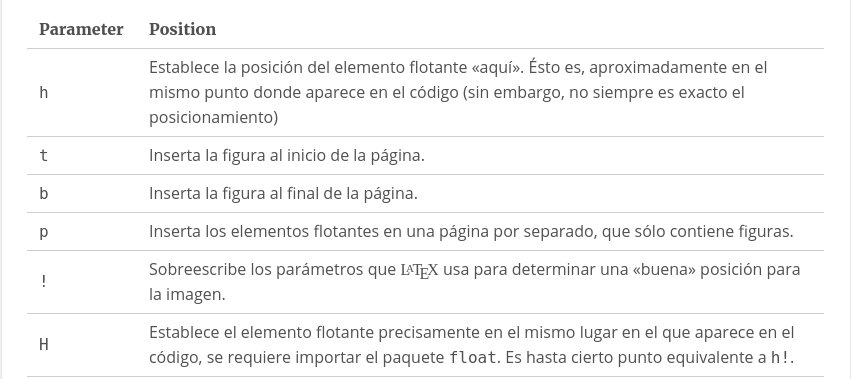
\includegraphics[scale=.7]{img/argumentos}
	\caption{En la imagen se puede ver un avion tipo X.}|
	\label{fig:avion}
\end{figure}

Ahora vamos a ver cómo agregar imágenes simples en un documento. Como se puede ver en la Figura \ref{fig:avion} tenemos un vortice de punta de herradura.Ahora vamos a ver cómo agregar imágenes simples en un documento. Como se puede ver en la Figura \ref{fig:avion} tenemos un vortice de punta de herradura.Ahora vamos a ver cómo agregar imágenes simples en un documento. Como se puede ver en la Figura \ref{fig:avion} tenemos un vortice de punta de herradura.Ahora vamos a ver cómo agregar imágenes simples en un documento. Como se puede ver en la Figura \ref{fig:avion} tenemos un vortice de punta de herradura.Ahora vamos a ver cómo agregar imágenes simples en un documento. Como se puede ver en la Figura \ref{fig:avion} tenemos un vortice de punta de herradura.Ahora vamos a ver cómo agregar imágenes simples en un documento. Como se puede ver en la Figura \ref{fig:avion} tenemos un vortice de punta de herradura.Ahora vamos a ver cómo agregar imágenes simples en un documento. Como se puede ver en la Figura \ref{fig:avion} tenemos un vortice de punta de herradura.Ahora vamos a ver cómo agregar imágenes simples en un documento. Como se puede ver en la Figura \ref{fig:avion} tenemos un vortice de punta de herradura.Ahora vamos a ver cómo agregar imágenes simples en un documento. Como se puede ver en la Figura \ref{fig:avion} tenemos un vortice de punta de herradura.Ahora vamos a ver cómo agregar imágenes simples en un documento. Como se puede ver en la Figura \ref{fig:avion} tenemos un vortice de punta de herradura.Ahora vamos a ver cómo agregar imágenes simples en un documento. Como se puede ver en la Figura \ref{fig:avion} tenemos un vortice de punta de herradura.Ahora vamos a ver cómo agregar imágenes simples en un documento. Como se puede ver en la Figura \ref{fig:avion} tenemos un vortice de punta de herradura.Ahora vamos a ver cómo agregar imágenes simples en un documento. Como se puede ver en la Figura \ref{fig:avion} tenemos un vortice de punta de herradura.

\begin{figure}
	\centering
	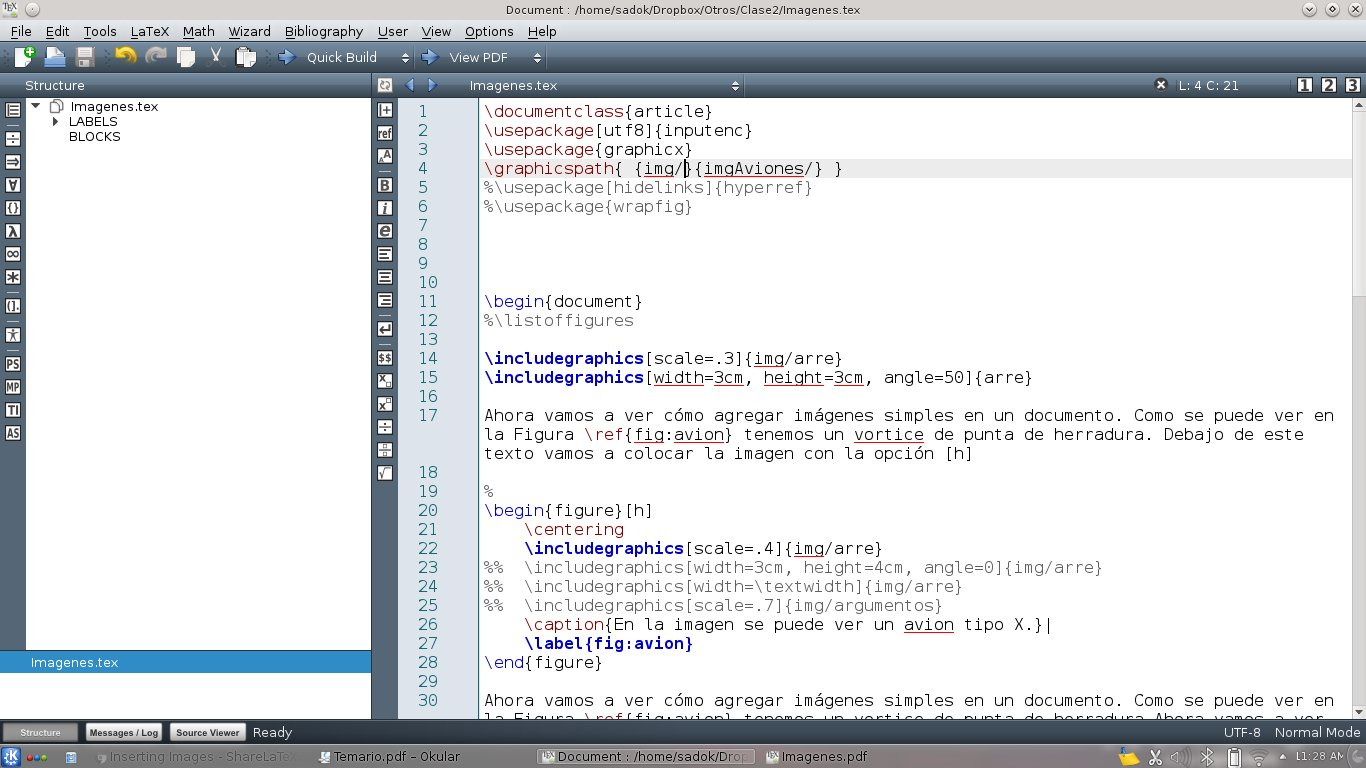
\includegraphics[scale=.2]{images/arre}
%%	\includegraphics[width=3cm, height=4cm, angle=0]{img/arre}
%%	\includegraphics[width=\textwidth]{img/arre}
%%	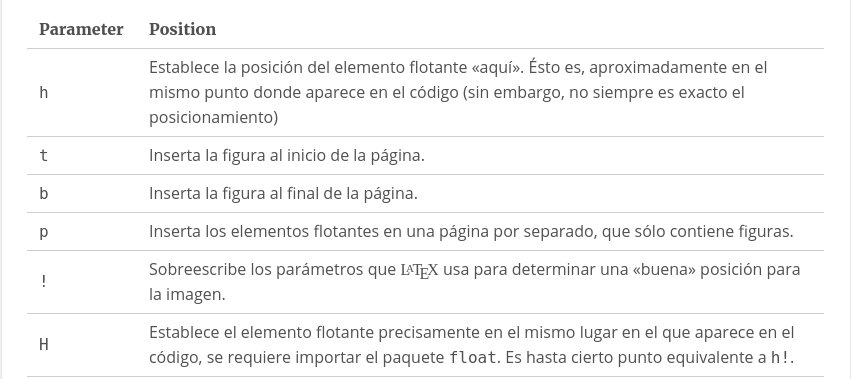
\includegraphics[scale=.7]{img/argumentos}
	\caption{Esta es la segunda Figura.}
	\label{fig:aviones}
\end{figure}
%
%
Una vez vista la imagen ahora vamos a ver las posiciones. On the other side, if you are only interested on certain values you can use the contour plot, you can use the contour plot, you can use the contour plot, you can use the contour plot, you can use the contour plot, you can use the contour plot, you can use the contour plot, like the one on the left.\\

\begin{wrapfigure}{r}{0.15\textwidth} %Figura a la derecha- Este valor es del espacio que va a alejar el texto de la img
    \centering
    \includegraphics[width=0.3\textwidth]{img/arre}
\end{wrapfigure}
 
On the other side, if you are only interested on certain values you can use the contour plot, you can use the contour plot, you can use the contour plot, you can use the contour plot, you can use the contour plot, you can use the contour plot, you can use the contour plot, like the one on the left.Una vez vista la imagen ahora vamos a ver las posiciones. On the other side, if you are only interested on certain values you can use the contour plot, you can use the contour plot, you can use the contour plot, you can use the contour plot, you can use the contour plot, you can use the contour plot, you can use the contour plot, like the one on the left.\\

\begin{wrapfigure}{l}{0.25\textwidth} %Figura a la derecha- Este valor es del espacio que va a alejar el texto de la img
    \centering
    \includegraphics[width=0.25\textwidth]{img/arre}
\end{wrapfigure}

Una vez vista la imagen ahora vamos a ver las posiciones. On the other side, if you are only interested on certain values you can use the contour plot, you can use the contour plot, you can use the contour plot, you can use the contour plot, you can use the contour plot, you can use the contour plot, you can use the contour plot, like the one on the left.\\

\begin{thebibliography}{99}

\bibitem{cookie} https://es.sharelatex.com/learn/Inserting\_Images

\end{thebibliography}

\end{document}